\chapter{Proposed Algorithm}\label{ch:algorithm}
The objective of the human counting algorithm is clarified as following.

The detector should be capable of detecting human objects in a relative large range of temperature, because the detected temperature of human body depends heavily on the wearing clothes and individual body condition. The detector should be sensitive to detect a human that is slightly hotter than the ambient environment. Meanwhile, fluctuation of the environment temperature should be taken into account carefully. A pixel value that is just above the ambient temperature in a cool morning would be regarded as active, but the same value would probably be a noise reading in the afternoon of the same day.

The human body tracker should work properly for single human events, as well as more complicated events when multiple people interact with the door, including but not limited to: two people traversing parallel, traversing sequential but with a narrow distance, traversing in opposite direction, or one person standing still and another pass by. The tracker should not assume that the detected pixel blobs are separated perfectly, and should be able to track two once separate blobs when they merge, as well as assign the correct labels when they split again.

And finally, the time consumption of one single image processing must be constraint within 100ms because the camera runs at 10fps. Considering that other tasks, such as data reading from camera register and publishing MQTT messages, also takes CPU process time, the time window left for detecting and tracking is merely around 50ms.
%TODO: Add a picture with the steps of the algorithm
\section{Blob Detection} \label{sec:detect}
\subsection{Active Pixel Detection}
Before the actual fore- and background segmentation, an early detection process is conducted on the $8\times8$ coarse image to see whether there is a potential heat source in the camera view. We check if there are at least three pixels having a value $1.5^\circ C$ higher than the room temperature. The parameters are chosen based on the following calculation. When installed at a height of $2.5m$, the Grideye sensor covers an area of about $8m^2$, which is much larger than a human body. However, when a human enters the camera view, the projection of his body on the image is caused by the horizontal plane of the shoulders, which is much higher than the ground and closer to the camera. Assuming the average shoulder height is $1.4m$, the real coverage of the camera is $4m^2$, only half of the ground area that it can cover. We assume the horizontal plane of a human body is not less than $2dm^2$, which amounts to at least three pixels in the image frame. The threshold $1.5^\circ C$ above the room temperature is chosen to filter out the sensor noise, we denote this threshold as $T_{lb}$ (low boundary).
%todo: 大概的示意图
\subsection{Segmentation Threshold Determination}
To separate human objects from the background, we follow the idea of calculating a global threshold from image statistic values, which is inspired by \cite{virtualtrack} and \cite{jeong2014probabilistic}. The threshold $T_{th}$ is calculated by the following formula (\autoref{eq:detectionthreshold}), where Max is the maximum pixel value among all 64 pixels and SD is the standard deviation. By thresholding, the original raster image is linearly interpolated to a resolution of $71\times71$ by inserting nine pixels between each pixel to avoid numeric issues in the following segmentation. The same resolution is also used by \cite{virtualtrack} and \cite{mika}.
\begin{equation}\label{eq:detectionthreshold}
  T_{th} = max\{Max - 4\times SD, T_{lb}\}
\end{equation}

The formula is simple but effective. The result is shown in \autoref{fig:detectioninterpolate}. Comparing image (c) and (e), it is apparent that the interpolation step is necessary to preserve more information from the original image and obtain a smooth shape of the object.
\begin{figure}
  \centering
  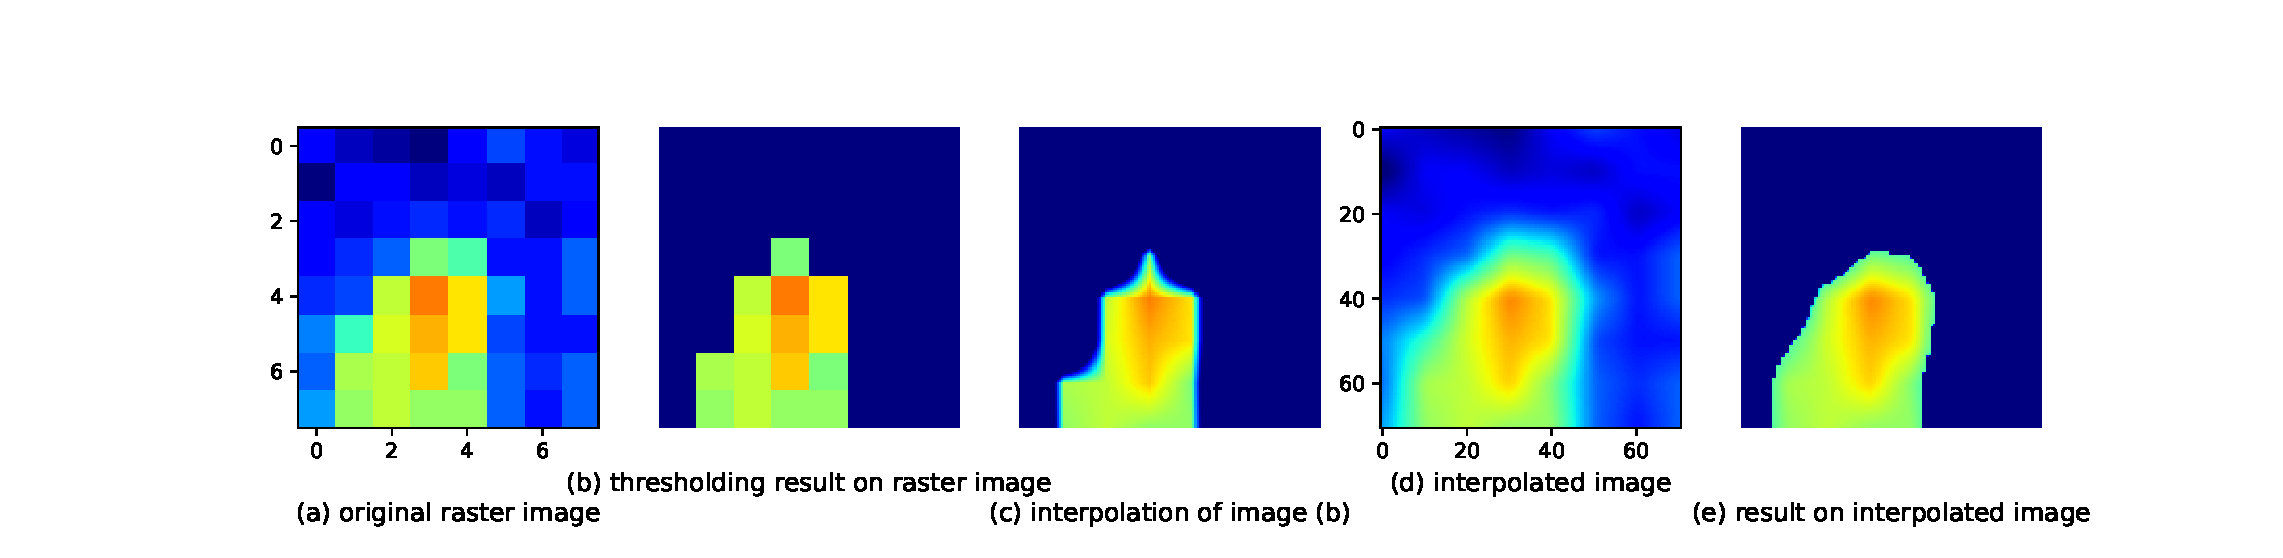
\includegraphics[width=\textwidth]{figures/detect_interpolate.eps}
  \caption{Result given by \autoref{eq:detectionthreshold}, the interpolated image preserves more details after thresholding.}\label{fig:detectioninterpolate}
\end{figure}

\subsection{Spacial Active Pixel Filter}
We notice that a single global threshold cannot separate two close objects very well. When two human stand close to each other, the small region between them will have a temperature higher than the room temperature because the pixel value results from a size-weighted average of both objects and background. This effect creates fake active pixels in the binary mask, see the first row in \autoref{fig:detectionspatialfilter}.

Therefore, pixels higher than the threshold but with hotter pixels nearby should be ignored because they originates from those hotter pixels and do not represent the true heat distribution. Reversely speaking, only those pixels that are hotter than its surrounding, namely local maxima pixels, contain valid information. We use the average filtered image as a spatial filter. After experiments on the collected image frames, a kernel size of 36 is chosen (half of the frame width). The value of every pixel in the filter is calculated by averaging a $36\times36$ neighbourhood surrounding that pixel location in the original image. Afterwards, the original image is compared with the filter pixel-wise, and only those pixels with a value higher than its filter counterpart will be kept. \autoref{fig:detection3d} shows the process in a surface plot, it shows the same image frame from \autoref{fig:detectionspatialfilter}. The threshold calculated from \autoref{eq:detectionthreshold} is applied to the local maxima image. The result is shown in the second row of \autoref{fig:detectionspatialfilter}, it is clear that the bridge connecting two objects becomes much narrower, which is beneficial for recognition as there are two objects in the frame, instead of one single large object. Moreover, it is not necessary to eliminate the bridge completely as we have a feature extraction step, which will be discussed in the next section.
\begin{figure}
  \centering
  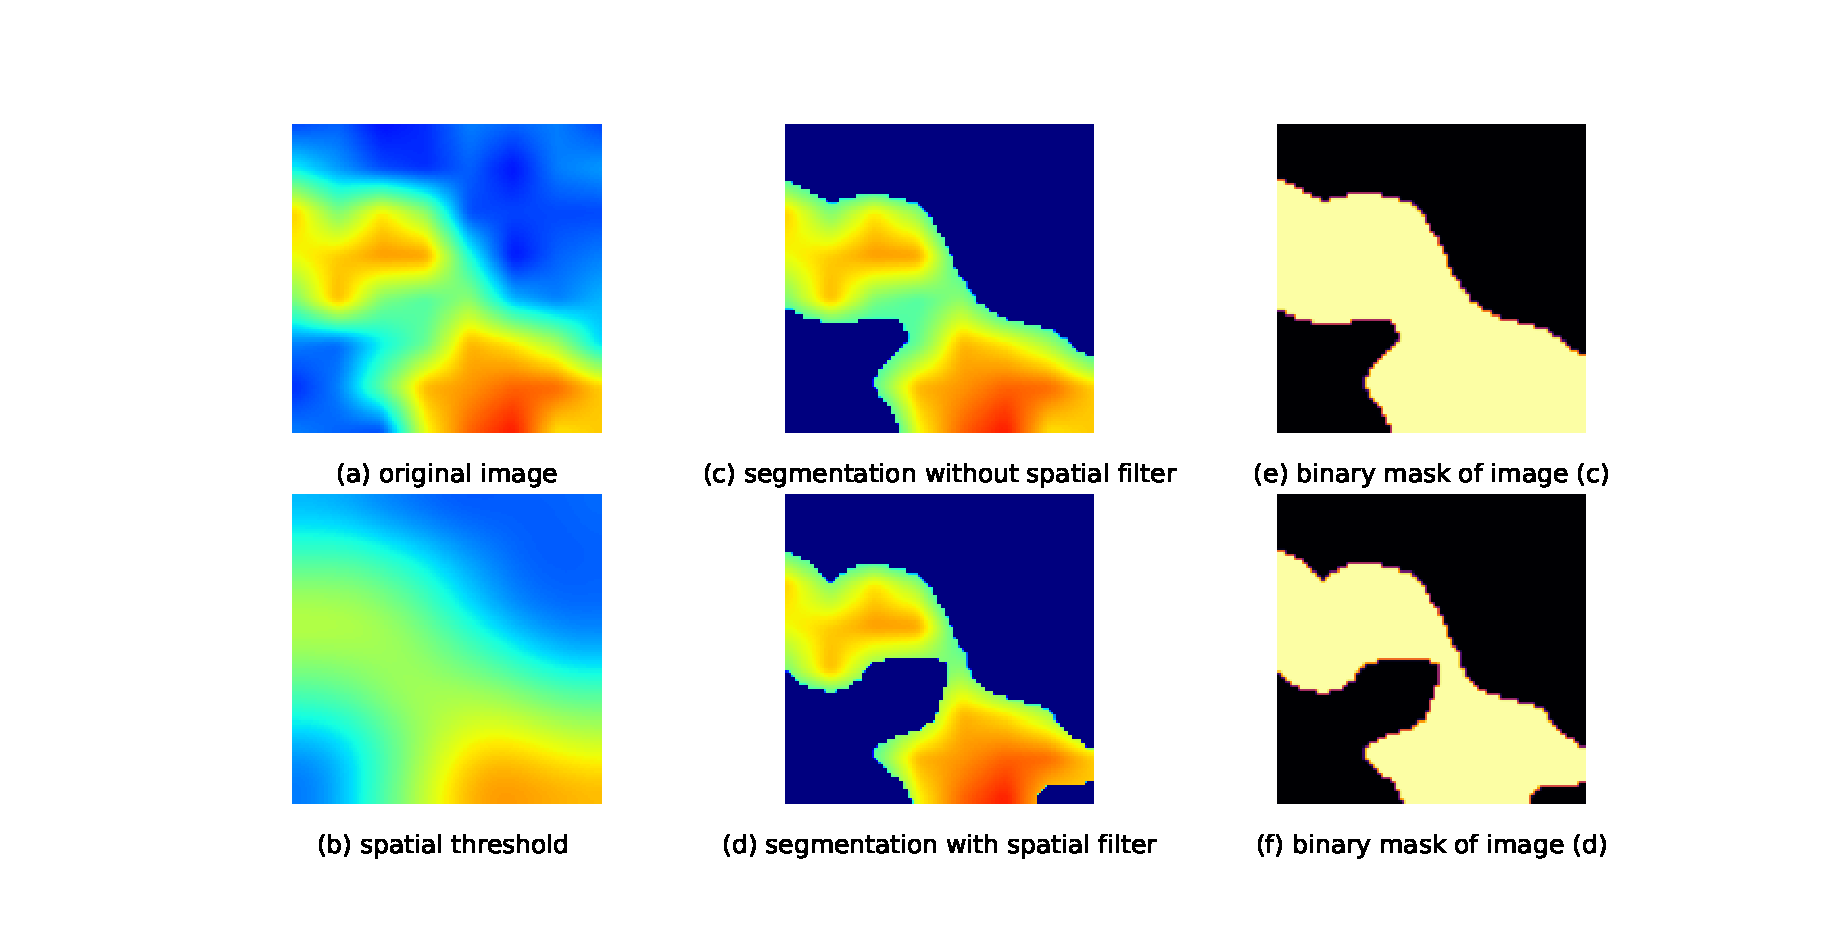
\includegraphics[width=\textwidth]{figures/detect_spatialfilter.eps}
  \caption{After introducing a spatial filter, the region between two objects are no longer marked as occupied.}\label{fig:detectionspatialfilter}
\end{figure}
%TODO: 更换图片
\begin{figure}
  \centering
  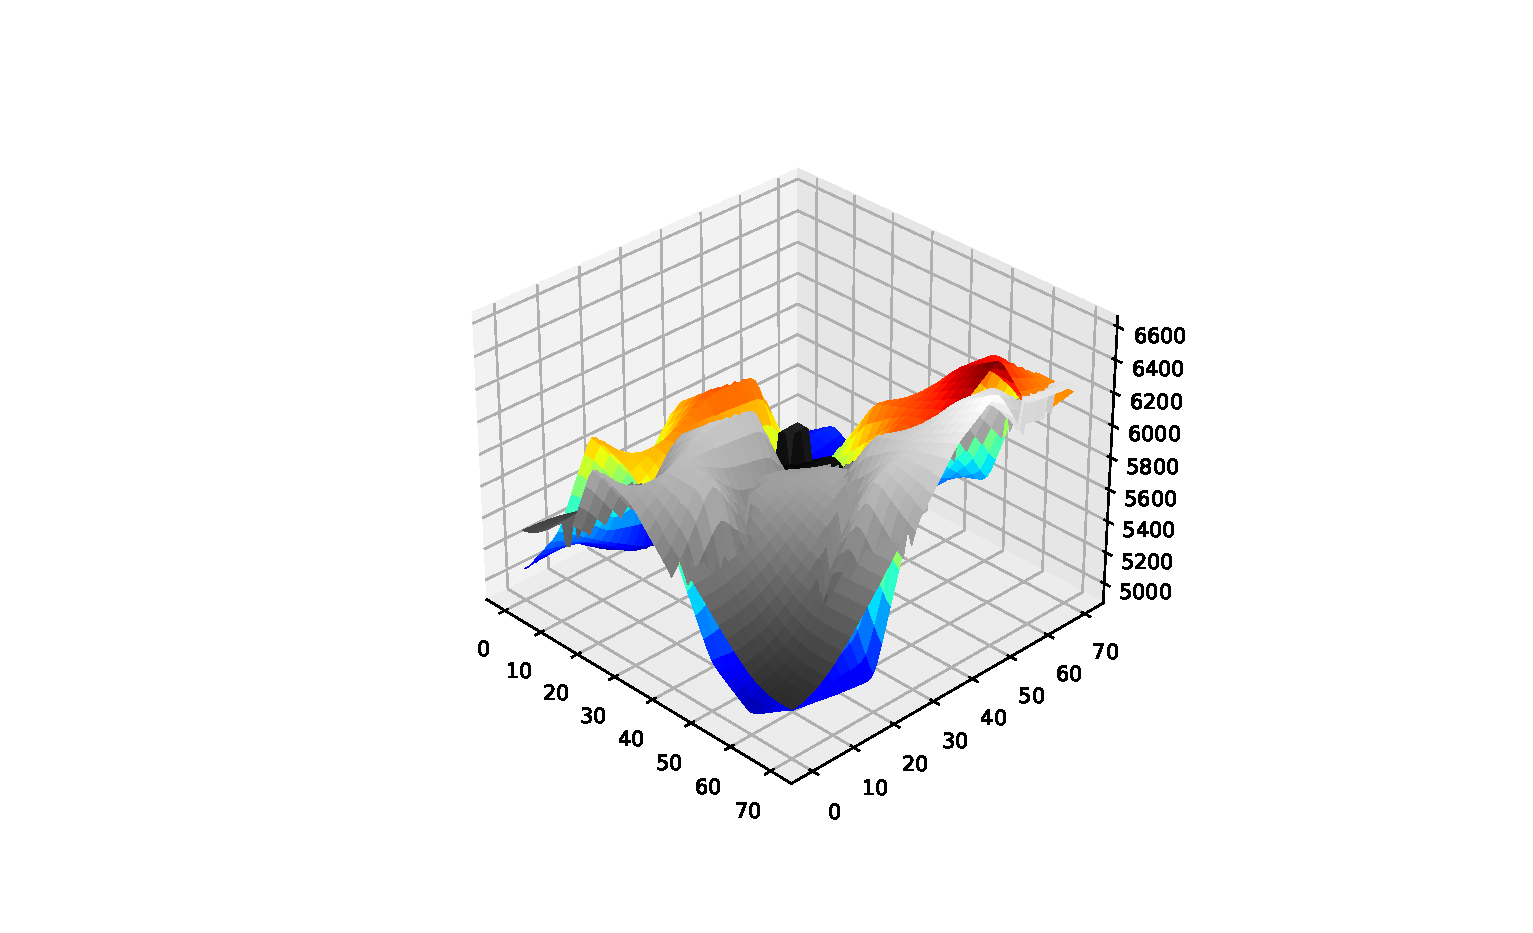
\includegraphics[width=\textwidth]{figures/detect_filterthres.eps}
  \caption{Only those pixels hotter than the region average are kept. The gray layer is the average filtered image and the colored layer is the original image.}\label{fig:detection3d}
\end{figure}

Moreover, this method outperforms simply increasing the global threshold because it has a better generalization ability for different body temperature. Though the aforementioned pixel bridge could also be eliminated by increasing the global threshold, we find that the threshold must be set very high to obtain a similar result. \autoref{fig:detectioncompare} shows the result of both method in two real scenarios. The first row shows the same frame in \autoref{fig:detectionspatialfilter}, where a tight global threshold of $Max-1.5\times SD$ turns out to be even better than our proposed method. However, when two human with distinct temperature occur in the same frame, the hotter object raises the global threshold with a higher $Max$ pixel value. The threshold will be too high for the cooler object, and only the hotter object is detected.
\begin{figure}
  \centering
  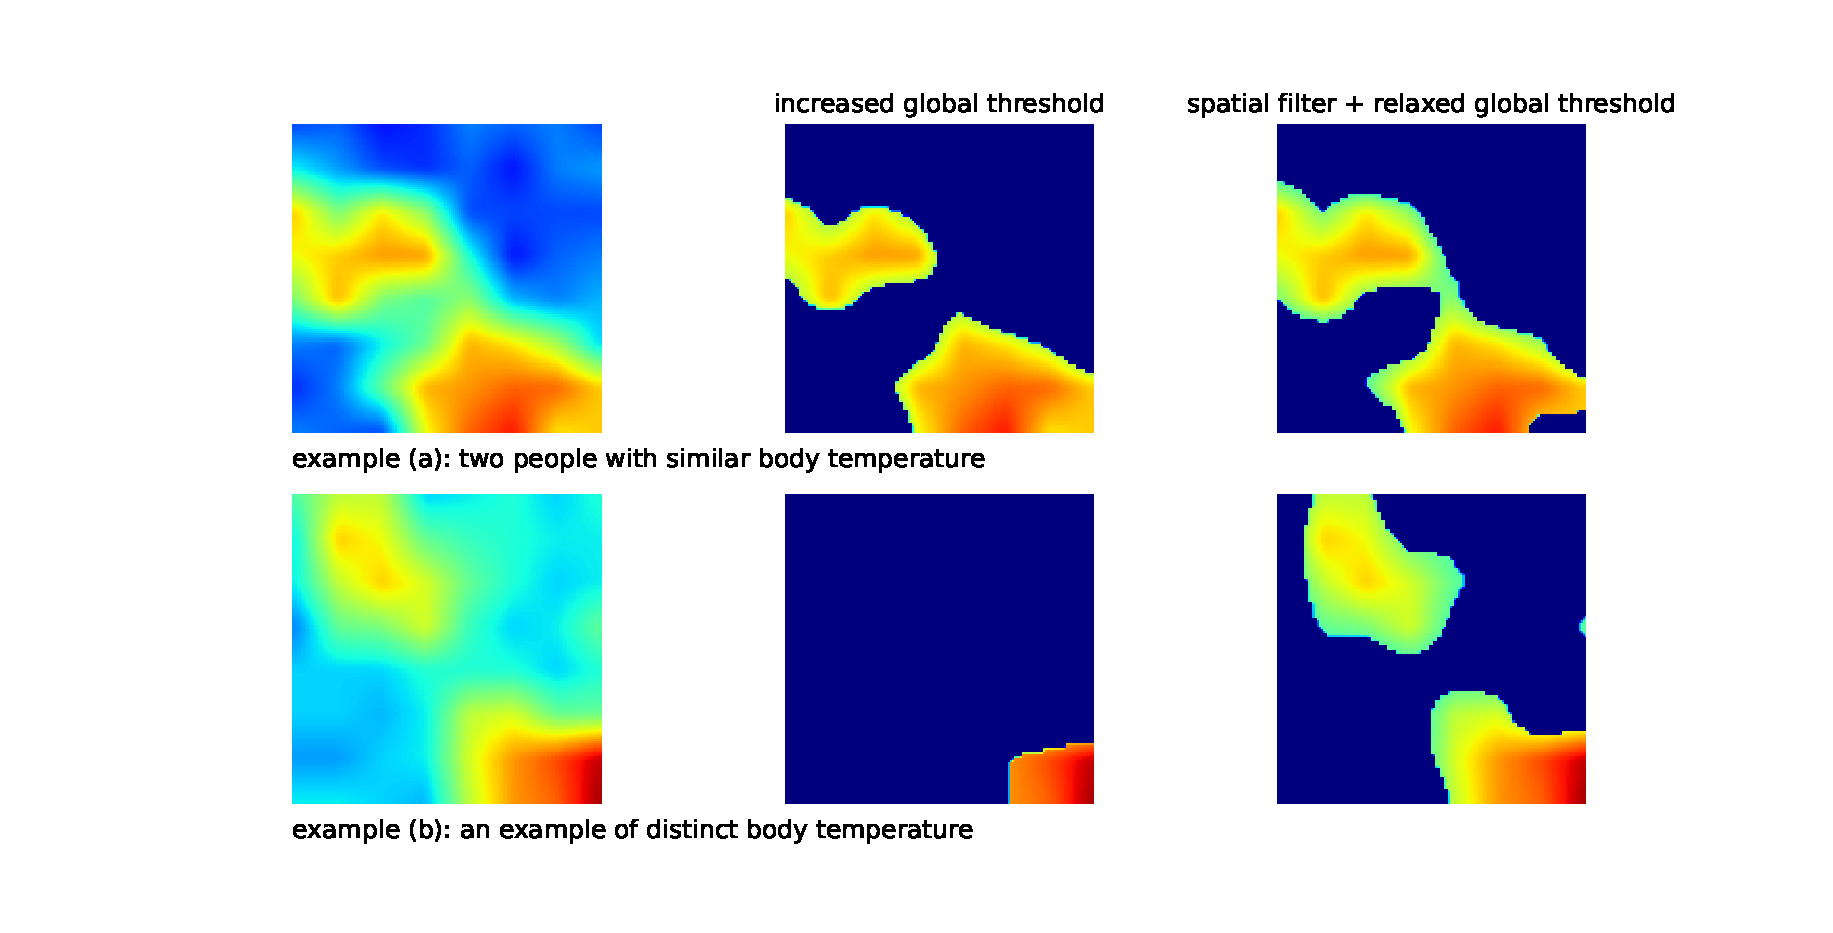
\includegraphics[width=\textwidth]{figures/detect_compare.eps}
  \caption{The middle column shows the segmentation result by a global threshold of $Max-1.5\times SD$, the right column shows the result by the proposed method. Both objects are detected whether they have distinct body temperature.}\label{fig:detectioncompare}
\end{figure}

With respect to the implementation, a convolution kernel with size $36\times36$ is too slow to meet the demand of realtime performance. For a $M\times N$ image and a $K\times K$ kernel, the time complexity of average pooling is $M\cdot N\cdot K^2$. Though the time complexity could be reduce to $M\cdot N\cdot K$ by separating the 2-dimensional kernel to two $36\times 1$ 1-dimensional kernels, the time consumption is still not satisfying. Our experiments show that on a ESP32 processor with 160MHz frequency, it takes seconds to convolve with a 2d kernel and about 70 milliseconds to convolve with two 1d kernels. We boost the processing performance by replacing the average polling algorithm with a summed-area table \cite{summedareatables}, which reduce the time complexity to $M\cdot N$.

A summed-area table, or sometimes called an integral image, is an image with the same size of the original image, where every pixel's value is the summation of all the pixels on the top-left of it. A summed-area table could be calculated efficiently from the original image in a recursive way, because the value of each pixel only depends on three pixels above, on the left and on the left-top of it.
To calculate the average value of a sub-region in the original image, only four corner points of that region in the summed-area table are needed. \autoref{fig:summedareatable} demonstrates how a summed-area table is calculated and used.

\begin{figure}
  \centering
  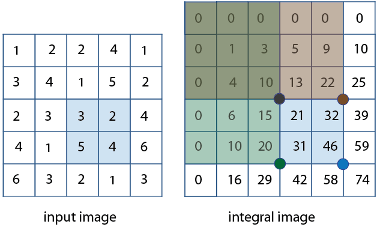
\includegraphics[width=0.6\textwidth]{figures/summedareatable.png}
  \caption{The basic idea of a summed-area table. Credit: \cite{summedareatableimage}}\label{fig:summedareatable}
\end{figure}


For comparison, the summed-area table based average filter takes only around 2ms for a single frame with the same processor configuration.
\subsection{Hole Filling}
Another common issue in segmentation is caused by the hair isolation of the head. From a top view, the human body is typically represented as an ellipse containing the head, two shoulders and partial upper torso. Ideally, the blob representation should have the highest temperature at the center and have a descent gradient to the margin. Unfortunately, a lower temperature is often observed in the blob center because a person's hair decays the heat emissivity. This will create a hole in the final binary blob and cause confusion, see \autoref{fig:detectionhole}.
\begin{figure}
  \centering
  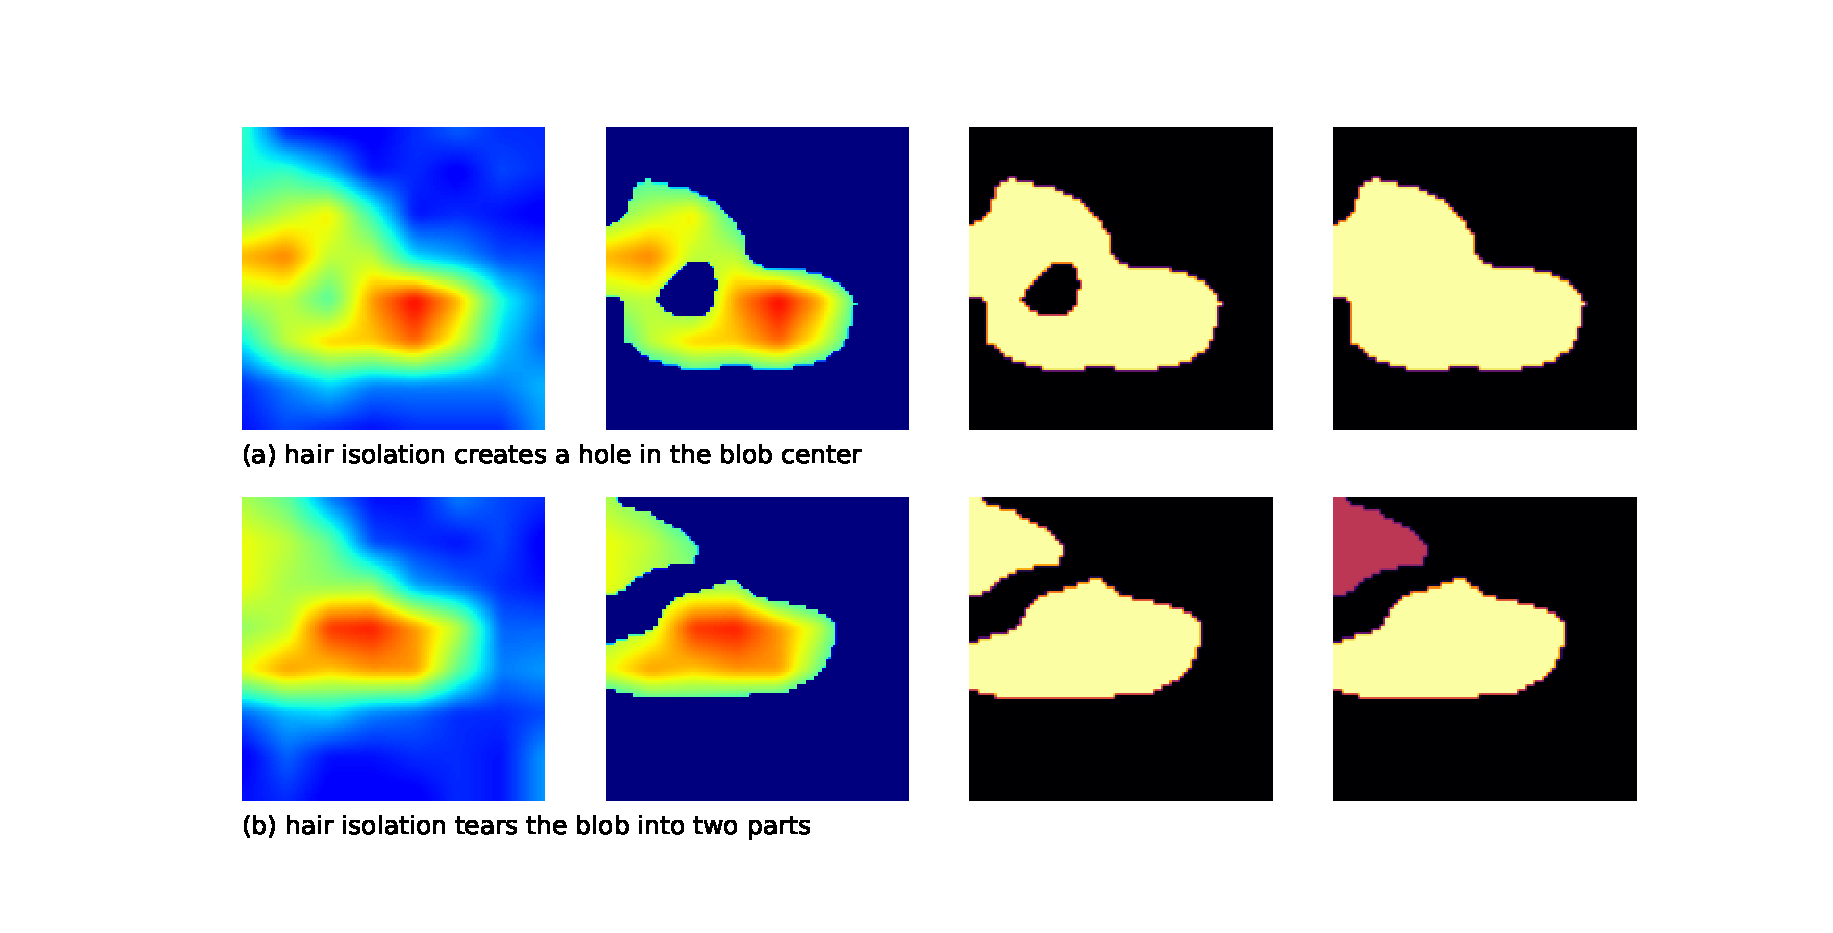
\includegraphics[width=\textwidth]{figures/detect_hole.eps}
  \caption{Two incorrect detection caused by hair isolation. The former could be fixed in detection layer, but the latter is left for tracking layer.}\label{fig:detectionhole}
\end{figure}

Since our detection method does not include any prior knowledge about the blob shape, any pixel that is cooler than the threshold will be regarded as background. There is no way to distinguish whether a pixel is truly a background pixel or belongs to a human but isolated. Moreover, because the hair is closer to the camera and has a large proportion in the blob presentation, the isolated region could be very large and even deteriorate the detection result.

If the hair isolation only creates a hole and the binary blob is still a connected domain, the hole could be filled with the flood-fill algorithm. Starting from the top-left pixel of the image, every connected background pixel is marked as occupied until there is no connected background pixel anymore. When there is a hole in the blob, the hole pixels are the only background left because they are surrounded by occupied pixels and are not reachable from a border background pixel. Then the processed binary mask will be logically reversed and merged with the original image. The final result is a blob representation without holes.

Nevertheless, if the hair isolation region is too large, the original blob will be separated into two parts, see the second row in \autoref{fig:detectionhole}. In this situation, even a human observer cannot distinguish whether it is a large person or two smaller people standing close by watching a single frame. A conclusion can only be drawn by taking previous frames into account. We decide not to solve this issue in the detection layer and leave it for the tracking layer. 